\section{Solving the Bellman Equation}
\label{sec:81models}

\minitoc[-0.5mm]{76mm}{4}

\noindent
In this section, we give a mathematical framework for
dynamic portfolio choice models,
briefly mention related literature, and
explain where B-splines on sparse grids come into play.
\Cref{tbl:glossaryFinance} summarizes the symbols
that are introduced in this chapter.
Rust provides a more detailed introduction to
dynamic portfolio choice models \cite{Rust18Dynamic}.

\begin{table}
  \setnumberoftableheaderrows{0}%
  \newcommand*{\vph}{%
    \vphantom{\printnotationsymbol{\buysell}}%
  }%
  \newcommand*{\pnst}[1]{%
    \printnotationsymbol{#1}\vph&\printnotationtext{#1}%
  }%
  \newcommand*{\pnsta}[1]{%
    \printnotationsymbol{#1}\vph&\multicolumn{3}{l}{\printnotationtext{#1}}%
  }%
  \begin{tabular}{%
    >{\kern\tabcolsep}=l+l<{\kern4.5mm}+l<{\kern-1.5mm}+l%
    <{\kern4.5mm}+l<{\kern-1mm}+l<{\kern\tabcolsep}%
  }
    \toprulec
    \pnst{t}&            \pnst{\wealth}&      \pnst{\utilityfcn}\\
    \pnst{\state}&       \pnst{\consume}&     \pnst{\statefcn}\\
    \pnst{\policy}&      \pnst{\bond}&        \pnst{\valuefcn}\\
    \pnst{\stochastic}&  \pnsta{\cetvalueintp}\\
    \pnst{\riskav}&      \pnst{\stock}&       \pnst{\optpolicyfcn}\\
    \pnst{\patience}&    \pnst{\buysell}&     $\hat{({\cdot})}$&Normalized quantity\\
    \pnst{\bondreturn}&  \pnst{\stockreturn}& \pnst{\wealthratio}\\
    \pnst{\tac}&         \pnsta{\weightedeulererror}\\
    \bottomrulec
  \end{tabular}%
  \caption[Glossary for dynamic portfolio choice models]{%
    Glossary of the notation for dynamic portfolio choice models.%
  }%
  \label{tbl:glossaryFinance}%
\end{table}



\subsection{Bellman Equation}
\label{sec:811bellmanEquation}

\paragraph{Utility maximization}

\usenotation{t}
In the following, dynamic portfolio choice models aim to maximize the expected
\term{discounted time-additive utility} over the lifetime of the individual,
where the terminal utility is derived solemnly from consumption
(i.e., no inheritance motive).
If we neglect stochastic factors, then these models solve
\begin{equation}
  \label{eq:utilityMaximization}
  (\optpolicyfcn_0, \dotsc, \optpolicyfcn_T)
  = \vecargmax_{\policy_0, \dotsc, \policy_T}
  \sum_{t=0}^T \patience^t \utilityfcn(\consume_t(\state_t, \policy_t))
  \quad\text{s.t. specific constraints.}
\end{equation}
Here, $\state_t \in \clint{\*0, \*1} \subset \real^d$ and
$\policy_t \in \real^{m_{\policy}}$
are the state%
\footnote{%
  We assume that each state variable $\stateentry_{t,o}$ ($o = 1, \dotsc, d$)
  is bounded, since the state space will be discretized with sparse grids.
  Without loss of generality, we may then assume that
  $\state_t \in \clint{\*0, \*1}$.
  If some state variables are unbounded in reality,
  then extrapolation is necessary,
  which will be explained in \cref{sec:825interpolation}.%
}
and policy of time $t = 0, \dotsc, T$, respectively.
The constraints ensure that for instance, we do not spend more money
than we actually have.
Starting from a given initial state $\state_0$,
the state $\state_{t+1}$ of time $t+1$ can be computed from
$\state_0$ and $\policy_0, \dotsc, \policy_t$ with a
\term{state transition function} $(\state_t, \policy_t) \mapsto \state_{t+1}$.
As shown in \cref{fig:dynamicPortfolioChoice},
in each time step, a fraction of the available wealth is consumed
\term{(consumption $\consume_t$),}
which can be computed from the state $\state_t$ and the policy $\policy_t$.
The individuals rate the consumption with a \term{utility function}
$\utilityfcn(\consume_t)$.
A common choice for $\utilityfcn$ is the \term{\crra utility}
$\utilityfcn(\consume_t) \ceq c_t^{1-\riskav}/(1-\riskav)$
with the \term{risk aversion} $\riskav \in \real \setminus \{1\}$.
Positive and negative values of $\riskav$
correspond to risk-averse and risk-affine individuals, respectively.
The factor $\patience \in \pohint{0, 1}$ is the \term{patience}
or \term{time discount factor.}

\begin{SCfigure}
  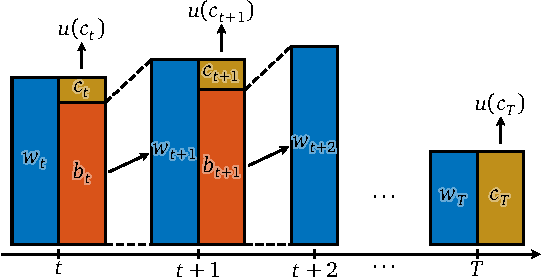
\includegraphics{dynamicPortfolioChoice_1}%
  \caption[Example of a dynamic portfolio choice model]{%
    Example of a dynamic portfolio choice model.
    The available wealth $\wealth_t$ is either
    invested into risk-free bonds ($\bond_t$) or consumed ($\consume_t$),
    resulting in utility $\utilityfcn(\consume_t)$.
    In the last time step $T$ \emph{(far right),}
    the optimal solution is to consume the whole wealth,
    if we do not take inheritance into account.%
  }%
  \label{fig:dynamicPortfolioChoice}%
\end{SCfigure}

\paragraph{Limitations of naive utility maximization}

When solving the utility maximization problem
in \cref{eq:utilityMaximization}, there are two issues.
First, solving \cref{eq:utilityMaximization} for all times $t$ at once
implies solving a $(T+1) m_{\policy}$-dimensional optimization problem,
which is usually computationally infeasible.
Second, \cref{eq:utilityMaximization} does not take stochastic variables
$\stochastic_t$ such as stock return rates into account.
These variables influence the state transition, i.e.,
$(\state_t, \policy_t, \stochastic_t) \mapsto \state_{t+1}$.
Consequently, $\state_{t+1}$ cannot be computed from $\state_0$ and
$\policy_0, \dotsc, \policy_t$ alone,
which complicates the solution of \cref{eq:utilityMaximization}
even for expected values.

\paragraph{Bellman principle}

To resolve the first issue,
Bellman's principle of optimality \cite{Bellman57Dynamic}
can be applied to problems like
\cref{eq:utilityMaximization} that are said to have
\term{optimal substructure.}
The principle states that the optimal policy for all times $t = 0, \dotsc, T$
is also optimal with respect to $t = 1, \dotsc, T$, i.e.,
{%
  \setlength{\abovedisplayskip}{6pt}%
  \begin{equation}
    \max_{\policy_0, \dotsc, \policy_T}
    \sum_{t=0}^T \patience^t \utilityfcn(\consume_t(\state_t, \policy_t))
    = \max_{\policy_0} \left(
      \utilityfcn(\consume_0(\state_0, \policy_0))
      + \patience \max_{\policy_1, \dotsc, \policy_T}
      \sum_{t=1}^T \patience^{t-1} \utilityfcn(\consume_t(\state_t, \policy_t))
    \right),
  \end{equation}%
}%
where we omitted the constraints for brevity.
The inner maximum problem over $\policy_1, \dotsc, \policy_T$
has the same structure as the problem on the \lhs.
With the \term{value function}
$\valuefcn_t\colon \clint{\*0, \*1} \to \real$,
$\valuefcn_t(\state_t) \ceq
\max_{\policy_t, \dotsc, \policy_T}
\sum_{t'=t}^T \patience^{t'-t}
\utilityfcn(\consume_{t'}(\state_{t'}, \policy_{t'}))$,
this can be rewritten as
{%
  \setlength{\belowdisplayskip}{9pt}%
  \begin{equation}
    \label{eq:simpleBellman}
    \valuefcn_0(\state_0)
    = \max_{\policy_0} \left(
      \utilityfcn(\consume_0(\state_0, \policy_0)) +
      \patience \valuefcn_1(\state_1)
    \right)
    \quad\text{s.t. specific constraints,}
  \end{equation}%
}%
where $\state_1$ is the result of the state transition
starting from $(\state_0, \policy_0)$.

\paragraph{General Bellman equation}

If we formulate \cref{eq:simpleBellman} for arbitrary times $t$ and
consider constraints, state transition, and stochastic variables,
we obtain the \term{Bellman equation:}
\begin{subequations}
  \setlength{\abovedisplayskip}{9pt}%
  \label{eq:generalBellman}
  \begin{gather}
    \valuefcn_t(\state_t)
    = \max_{\policy_t} \left(
      \utilityfcn(\consume_t(\state_t, \policy_t)) +
      \patience \expectation[t]{
        \valuefcn_{t+1}(\statefcn_t(\state_t, \policy_t, \stochastic_t))
      }
    \right),\quad
    t = 0, \dotsc, T,\\[-2mm]
    \policy_t \in \real^{m_{\policy}}\;\;\text{s.t.}\;\;
    \ineqconfun_t(\state_t, \policy_t) \le \*0,
  \end{gather}
\end{subequations}
where $\valuefcn_{T+1} :\equiv 0$ for simplicity,
$\statefcn_t\colon \clint{\*0, \*1} \times \real^{m_{\policy}} \times
\stochdomain \to \clint{\*0, \*1}$,
$(\state_t, \policy_t, \stochastic_t) \mapsto \state_{t+1}$,
is the \term{state transition function,}
$\ineqconfun_t\colon \clint{\*0, \*1} \times \real^{m_{\policy}} \to
\real^{m_{\ineqconfun}}$ is the \term{constraint function,} and
\begin{equation}
  \expectation[t]{
    \valuefcn_{t+1}(\statefcn_t(\state_t, \policy_t, \stochastic_t))
  }
  \ceq \int_{\stochdomain}
  \valuefcn_{t+1}(\statefcn_t(\state_t, \policy_t, \stochastic_t))
  P_{t,\stochastic}(\stochastic_t) \diff{}\stochastic_t
\end{equation}
with the probability density function
$P_{t,\stochastic}\colon \stochdomain \to \nonnegreal$ of $\stochastic_t$.%
\footnote{%
  While the state $\state_t \in \clint{\*0, \*1}$
  is continuous in this thesis,
  \term{Markov-chain discrete states} $\discrstate_t \in \discrstdomain$
  such as alive/dead
  (i.e., $\discrstdomain$ is the Cartesian product of finite sets)
  can be incorporated into \eqref{eq:generalBellman}.
  The objective function of $\valuefcn_t(\state_t, \discrstate_t)$ then equals
  $\utilityfcn(\consume_t(\state_t, \discrstate_t, \policy_t)) +
  \patience \expectation[t]{
    \valuefcn_{t+1}(\statefcn_t(\state_t, \discrstate_t,
    \policy_t, \stochastic_t), \discrstate_{t+1}) \mid \discrstate_t
  }$.%
}
We denote the location of the maximum of \eqref{eq:generalBellman}
as the optimal policy $\optpolicyfcn_t$,
which may be regarded as a function
$\optpolicyfcn_t\colon \clint{\*0, \*1} \to \real^{m_{\policy}}$,
$\state_t \mapsto \optpolicyfcn_t(\state_t)$.

\paragraph{Dynamic programming scheme}

The Bellman equation \eqref{eq:generalBellman} can be solved
backwards in time with a dynamic programming scheme.
Starting from the solution $\valuefcn_T$ and $\optpolicyfcn_T$
of time $T$, which is determined by maximizing the utility
for the terminal time step,
we can determine $\valuefcn_t$ and $\optpolicyfcn_t$
from $\valuefcn_{t+1}$ and $\optpolicyfcn_{t+1}$
for $t = T - 1,\, T - 2,\, \dotsc,\, 0$ with the Bellman equation.
This way, we only have to solve $T+1$ separate $m_{\policy}$-dimensional
optimization problems instead of a single large
$(T+1) m_{\policy}$-dimensional problem.
Often, the terminal solutions $\valuefcn_T$ and $\optpolicyfcn_T$
are explicitly known.
In our case, the optimal terminal solution is
to consume the whole wealth $\wealth_T$
(see \cref{fig:dynamicPortfolioChoice}).

\paragraph{Implementation and interpolation}

For the implementation of \eqref{eq:generalBellman},
we discretize the state space $\clint{\*0, \*1}$ into
$\ngp_t$ grid points $\state_t^{(k)}$, $k = 1, \dotsc, \ngp_t$,
and we tabulate the values of $\valuefcn_t$ and $\optpolicyfcn_t$
at $\state_t^{(k)}$ for all $t = 0, \dotsc, T$ and $k = 1, \dotsc, \ngp_t$.
However, in general, the next state
$\statefcn_t(\state_t^{(k)}, \policy_t, \stochastic_t)$ does not correspond
to a grid point $\state_{t+1}^{(k')}$,
which means that we cannot lookup the value of $\valuefcn_{t+1}$
at $\statefcn_t(\state_t^{(k)}, \policy_t, \stochastic_t)$.
Therefore, we have to interpolate $\valuefcn_{t+1}$
at the grid points, obtaining the interpolant $\valueintp_{t+1}$
as a result:
\begin{equation}
  \label{eq:gridBellman}
  \valueintp_t(\state_t^{(k)})
  = \max_{\policy_t} \left(
    \utilityfcn(\consume_t(\state_t^{(k)}, \policy_t)) +
    \patience \expectation[t]{
      \valueintp_{t+1}(\statefcn_t(\state_t^{(k)}, \policy_t, \stochastic_t))
    }
  \right),\quad
  k = 1, \dotsc, \ngp_t,
\end{equation}
where $\valueintp_{T+1} :\equiv 0$ for simplicity.
As $\valueintp_{t+1}$ on the \rhs is only an approximation to
$\valuefcn_{t+1}$, the values $\valueintp_t(\state_t^{(k)})$
on the \lhs are approximations, too.
Since we are mainly interested in the optimal policy decisions
$\optpolicyfcn_t$, we have to interpolate them as well, i.e.,
\begin{equation}
  \optpolicyintp_t(\state_t^{(k)})
  = \vecargmax_{\policy_t} \left(
    \utilityfcn(\consume_t(\state_t^{(k)}, \policy_t)) +
    \patience \expectation[t]{
      \valueintp_{t+1}(\statefcn_t(\state_t^{(k)}, \policy_t, \stochastic_t))
    }
  \right).
\end{equation}
Note that the employed grids for $\optpolicyintp_t$
may be different from the grids for $\valueintp_t$.



\subsection{Solution with B-Spline Surrogates on Sparse Grids}
\label{sec:812surrogates}

\paragraph{Sparse grids for dynamic models and related work}

As interpolation approaches for $\valuefcn_t$ based on full grids
suffer from the curse of dimensionality,
we want to use interpolation on spatially adaptive sparse grids instead.
Recently, sparse grids have found increasing interest in the
solution of dynamic models in finance
\multicite{Brumm17Using,Judd14Smolyak,Schober18Solving,Winschel10Solving}.
For example in \cite{Brumm17Using},
discrete choices in the value iteration are computed
using piecewise linear basis functions on spatially adaptive sparse grids.
Schober employs spatially adaptive sparse grids
for the interpolation of dynamic portfolio choice models,
but uses piecewise linear basis functions \cite{Schober18Solving}.
Judd et al.\ use global polynomials
on sparse Clenshaw--Curtis grids for the interpolation of
higher-dimensional economic models \cite{Judd14Smolyak}.

\paragraph{B-splines on sparse grids for dynamic portfolio choice models}

The shortcomings of the two approaches of piecewise linear functions
\multicite{Brumm17Using,Schober18Solving} or global polynomials
\cite{Judd14Smolyak} are evident:
Piecewise linear functions are not continuously differentiable,
impeding convergence of interpolation errors
(see \cref{sec:541interpolation}) and prohibiting the use
of gradient-based optimization methods to solve \cref{eq:gridBellman}.
The reason for the latter statement is that gradient-based optimizers require
the derivatives of the objective function of \cref{eq:gridBellman}
with respect to the entries $\policyentry_{t,j}$ of $\policy_t$
($j = 1, \dotsc, m_{\policy}$), i.e.,
\begin{equation}
  \begin{split}
    &\utilityfcn'(\consume_t(\state_t^{(k)}, \policy_t))
    \partialderiv{\partialdiff{}\policyentry_{t,j}}{c_t}\paren{
      \state_t^{(k)}, \policy_t
    }\\
    &{} + \patience \expectation[t]{
      \tr{
        \paren*{
          \gradient{\state_{t+1}}{\valueintp_{t+1}}\paren{
            \statefcn_t(\state_t^{(k)}, \policy_t, \stochastic_t)
          }
        }
      }
      \partialderiv{\partialdiff{}\policyentry_{t,j}}{\statefcn_t}\paren{
        \state_t^{(k)}, \policy_t, \stochastic_t
      }
    },
  \end{split}
\end{equation}
which involves the gradient
$\gradient{\state_{t+1}}{\valueintp_{t+1}}$ of the
value function interpolant $\valueintp_{t+1}$.
Gradient-based optimization methods do not converge fast
if this gradient is discontinuous.
Moreover, piecewise linear basis functions introduce
many additional local minima.
In contrast, global polynomials only work well on Clenshaw--Curtis grids
with Chebyshev-distributed nodes due to Runge's phenomenon.

In the following, we use higher-order B-splines as basis functions for
the interpolation of $\valuefcn_t$ and $\optpolicyfcn_t$.
This method has two advantages:
First, B-splines of degree $p > 1$ are continuously differentiable,
increasing the order of convergence and enabling
gradient-based optimization for solving \cref{eq:gridBellman}.
Second, B-splines are defined for arbitrary knot sequences,
leading to a greater flexibility when compared to global polynomials.
